\subsection{Detailed Relation Type Analysis}
\label{app:relation_type_study}




\begin{figure}[t]
\centering
 
\includegraphics[width=6in]{submissions/Jing2024/figures/experiments/relation_analysis/legend.pdf}
\\\vspace{-6mm}
\subfloat[\textit{Correctness} vs Head entity type]{
 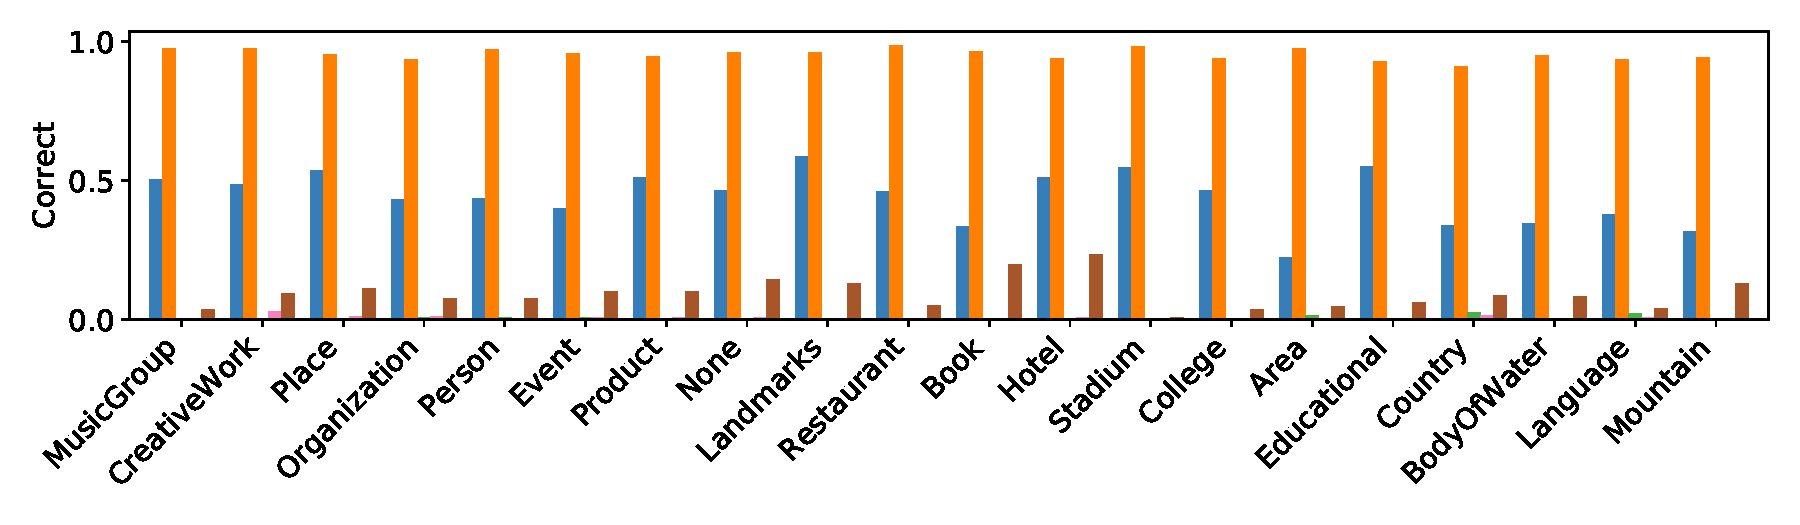
\includegraphics[width=5.5in]{submissions/Jing2024/figures/experiments/relation_analysis/correct_by_head_type.pdf}
 \label{fig:correct_by_head_type}
}\\

\includegraphics[width=5.5in]{submissions/Jing2024/figures/experiments/relation_analysis/legend.pdf}
\\\vspace{-6mm}
\subfloat[\textit{Correctness} vs Tail entity type]{
 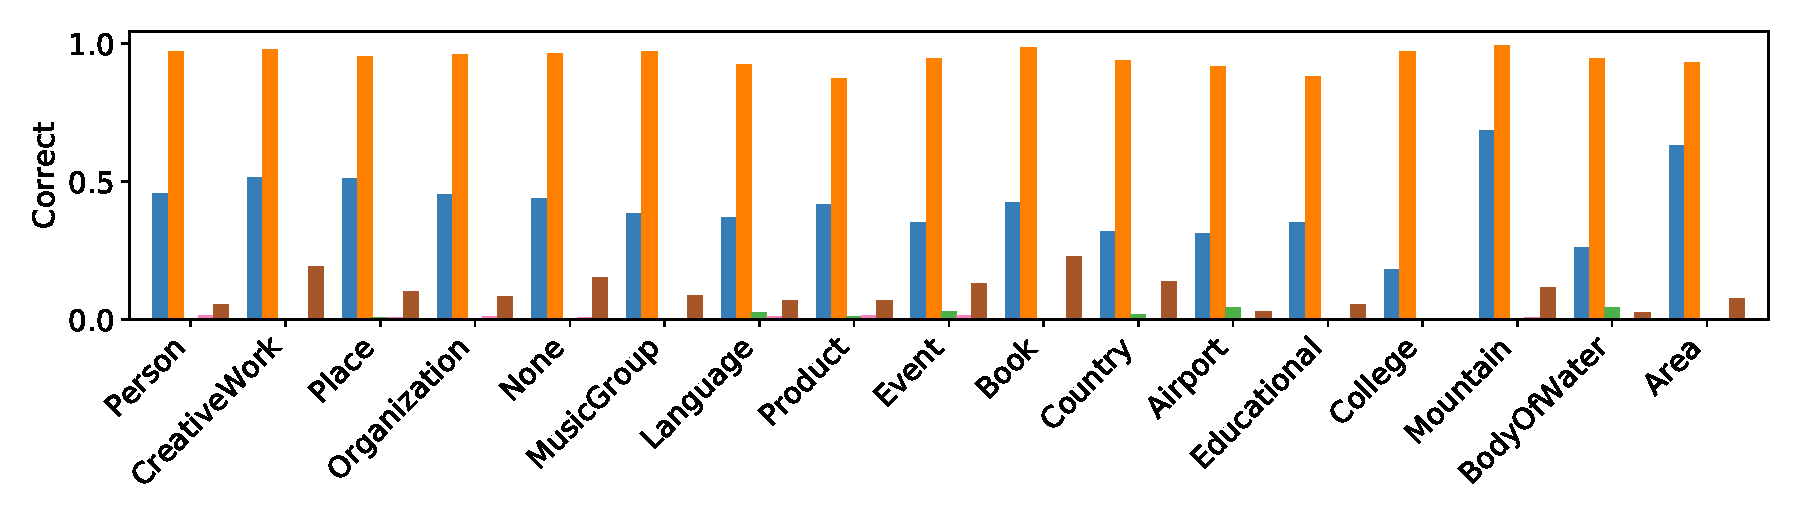
\includegraphics[width=5.5in]{submissions/Jing2024/figures/experiments/relation_analysis/correct_by_tail_type.pdf}
 \label{fig:correct_by_tail_type}
}
\caption{The LLM's \textit{correctness} with respect to head entity types and tail entity types}
\label{fig:correctness_by_type}
\end{figure}


\begin{figure}[t]
    \centering
 
\includegraphics[width=5.5in]{submissions/Jing2024/figures/experiments/relation_analysis/legend.pdf}
 \\\vspace{-6mm}
\subfloat[\textit{Truthfulness} vs Head entity type]{
 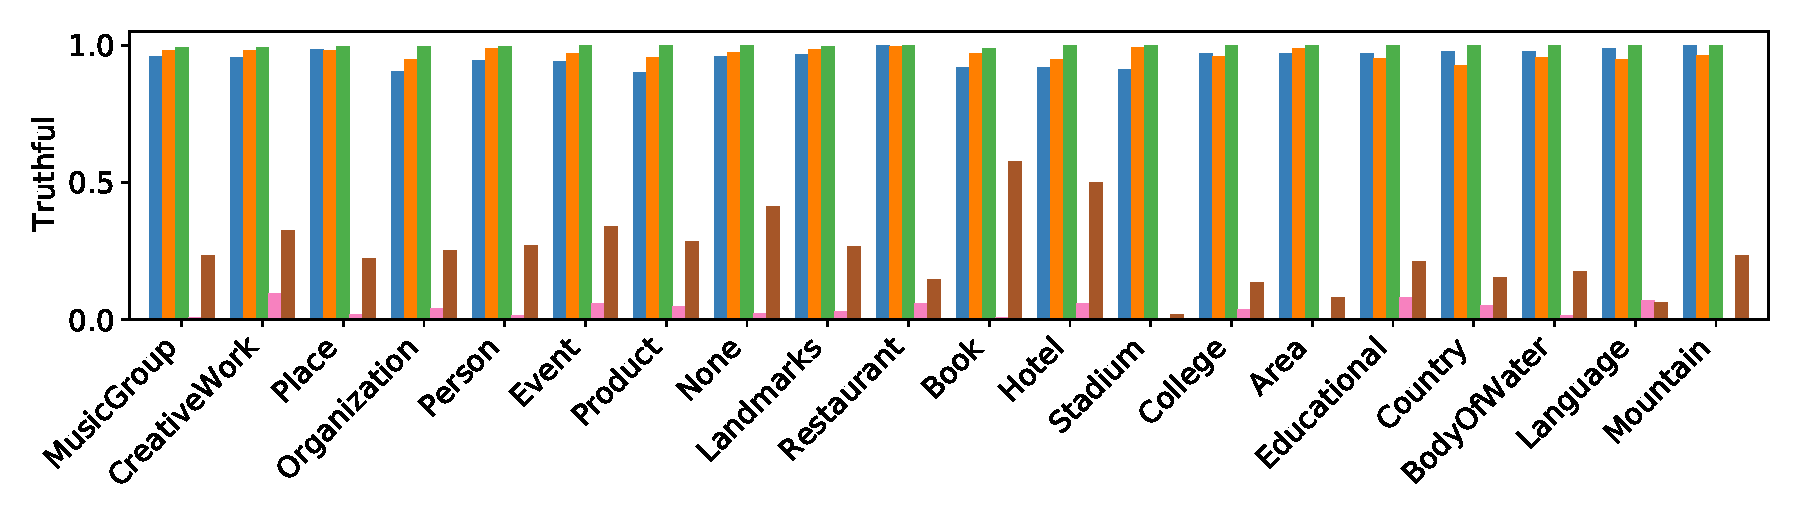
\includegraphics[width=5.5in]{submissions/Jing2024/figures/experiments/relation_analysis/truthful_by_head_type.pdf}
 \label{fig:truthful_by_head_type}
}\\

\includegraphics[width=5.5in]{submissions/Jing2024/figures/experiments/relation_analysis/legend.pdf}
\\\vspace{-6mm}
\subfloat[\textit{Truthfulness} vs Tail entity type]{
 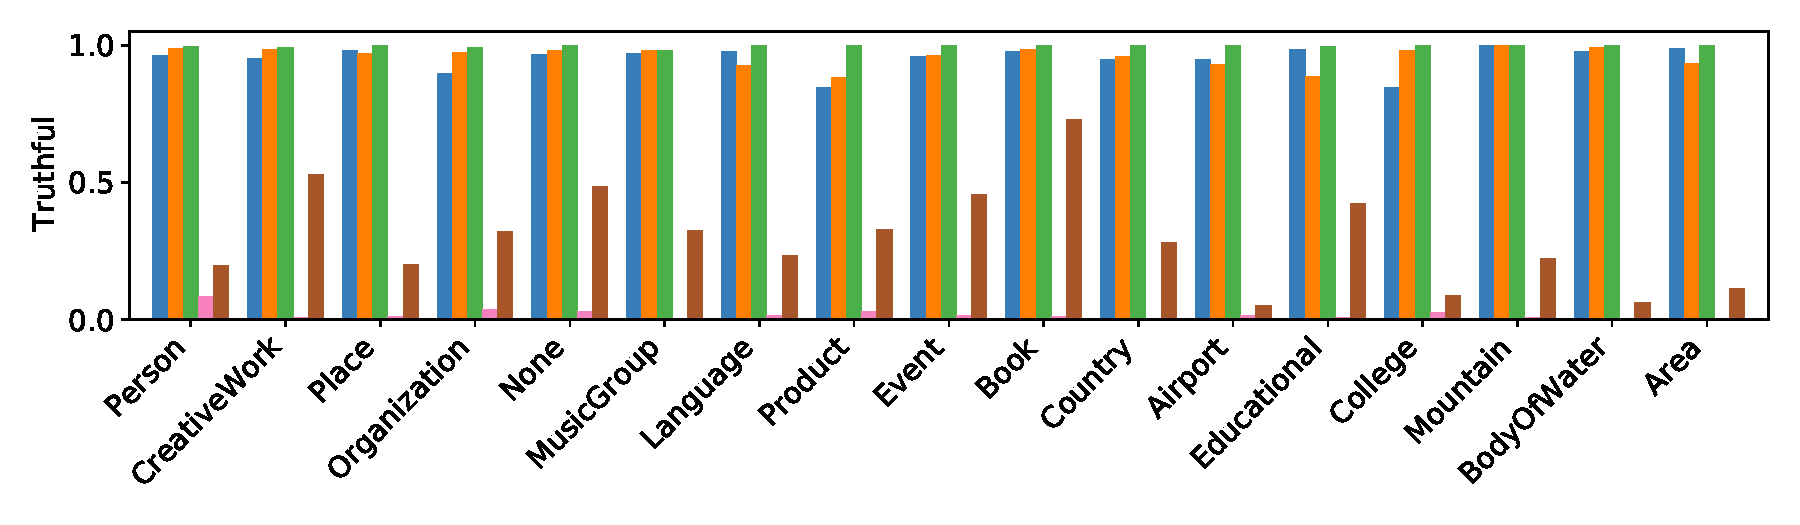
\includegraphics[width=5.5in]{submissions/Jing2024/figures/experiments/relation_analysis/truthful_by_tail_type.pdf}
 \label{fig:truthful_by_tail_type}
}
\caption{The LLM's \textit{truthfulness} with respect to head entity types and tail entity types}
\label{fig:truthfulness_by_type}
\end{figure}
\begin{figure}[t]
    \centering
    
\includegraphics[width=6in]{submissions/Jing2024/figures/experiments/relation_analysis/legend.pdf}
    \\\vspace{-6mm}
\subfloat[\textit{Informativeness} vs Head entity type]{
 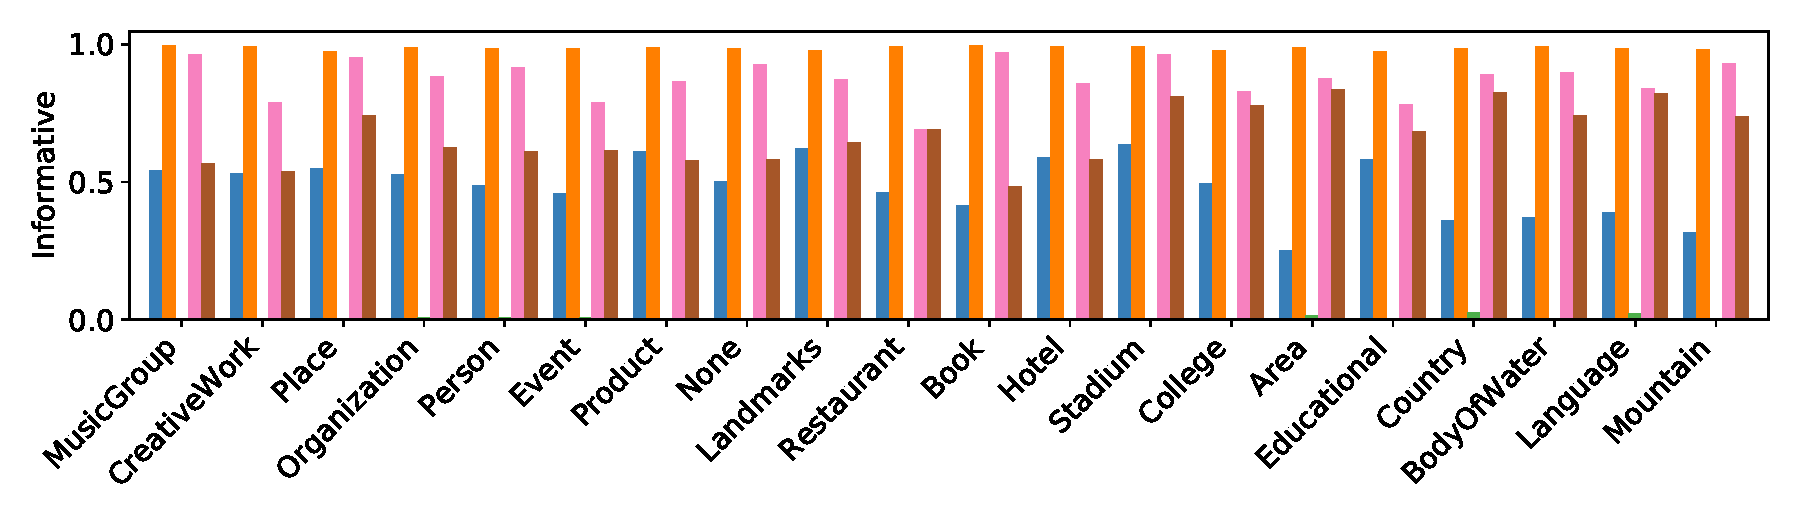
\includegraphics[width=5.5in]{submissions/Jing2024/figures/experiments/relation_analysis/informative_by_head_type.pdf}
 \label{fig:informative_by_head_type}
}\\

\includegraphics[width=5.5in]{submissions/Jing2024/figures/experiments/relation_analysis/legend.pdf}
\\\vspace{-6mm}
\subfloat[\textit{Informativeness} vs Tail entity type]{
 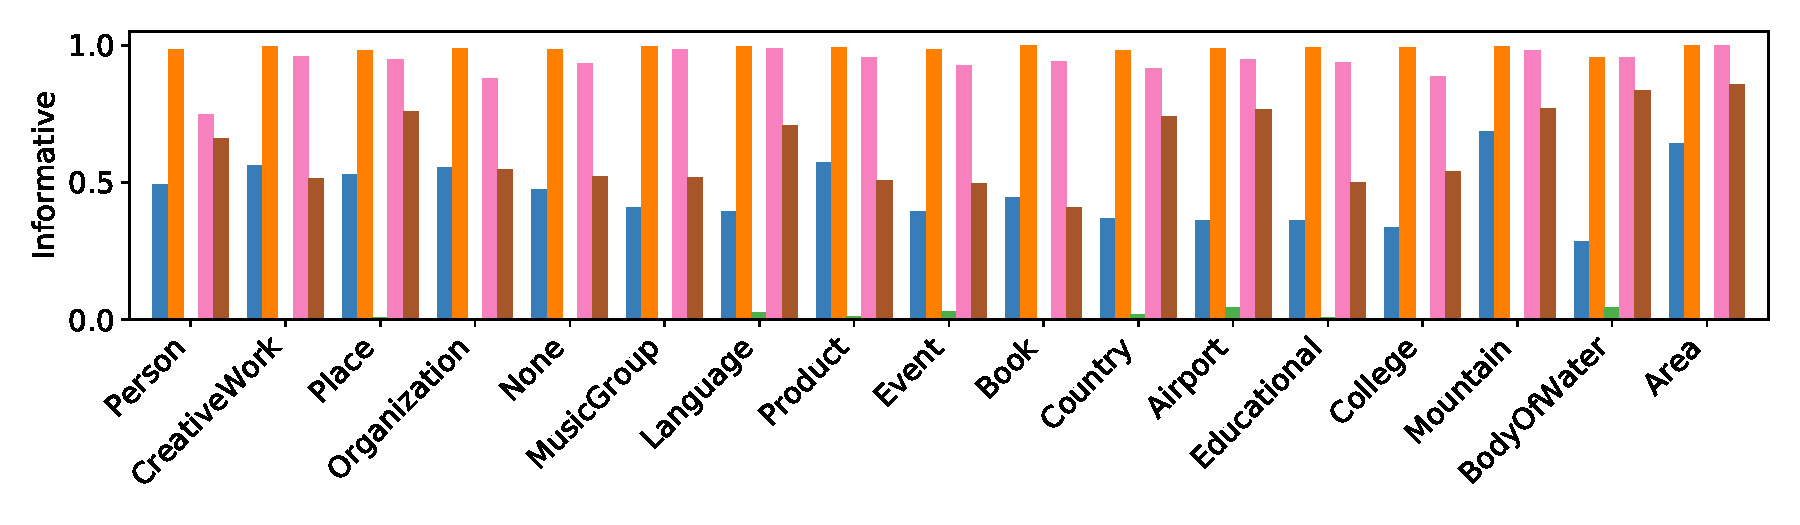
\includegraphics[width=5.5in]{submissions/Jing2024/figures/experiments/relation_analysis/informative_by_tail_type.pdf}
 \label{fig:informative_by_tail_type}
}
\caption{The LLM's \textit{informativeness} with respect to head entity types and tail entity types}
\label{fig:informativeness_by_type}
\end{figure}



\paragraph{Llama Family Analysis}
Across the LLaMA family, a progressive improvement in performance is observed from  7b to 13b. The 7b model shows decent performance across categories with a particular strength in the \textit{truthfulness}. However, its \textit{informativeness} and \textit{correctness} metrics show room for improvement, particularly in categories like Book, Hotel, and College, indicating a struggle to accurately provide informative and correct classifications in more nuanced or specific domains.

The LLaMA 13b model demonstrates a significant leap in performance, especially in \textit{informativeness} and \textit{correctness}, nearly reaching perfection across most categories. This jump can be attributed to the model's increased capacity, enabling it to understand and process the nuances of various entities better, resulting in remarkably high scores in nearly all categories, especially noticeable in MusicGroup, CreativeWork, and Place.

The LLaMA 70b results appear anomalous with extremely high \textit{truthfulness} scores but negligible \textit{informativeness} and \textit{correctness} across all categories. We suspect this discrepancy might be due to the model's knowledge awareness~\cite{ren2023investigating}, where the model might be less confident in its responses when the parameters are increased, leading to a higher proportion of ``I don't know" responses. This could explain the high \textit{truthfulness} scores but low \textit{informativeness} and \textit{correctness} metrics, as the model might be too cautious to provide definitive answers.

\paragraph{Gemma Family Analysis}
The Gemma models present an interesting contrast. The Gemma 2b model shows a tendency towards high \textit{informativeness} in certain categories like MusicGroup and Book but lacks behind significantly in \textit{truthfulness} and \textit{correctness} metrics. This suggests that while the model might be picking up on relevant information, it struggles to accurately validate the truth behind that information or its applicability to the queried entities.
The Gemma 7b model shows improvement in the \textit{truthfulness} metric compared to Gemma 2b, particularly noticeable in categories like Book and Hotel, and even surpasses LLaMA 7b in certain areas like None and Restaurant. However, it still significantly lags behind the LLaMA models, particularly LLaMA 13b, in both \textit{informativeness} and \textit{correctness}. The improved but still limited performance suggests that while Gemma 7b has a better grasp over the veracity of information compared to Gemma 2b, it still struggles with providing highly informative and correct outputs consistently across various entities.
